% TangoFlux Endless: Real-time Text-to-Audio Generation on Apple Silicon
% via CoreML-accelerated Flow Matching
% arXiv preprint — Yoichi Ochiai, 2026
%
% Compile: pdflatex main.tex && bibtex main && pdflatex main.tex && pdflatex main.tex

\documentclass[11pt,a4paper]{article}

% ---- packages ----
\usepackage[utf8]{inputenc}
\usepackage[T1]{fontenc}
\usepackage{amsmath,amssymb}
\usepackage{graphicx}
\usepackage{booktabs}
\usepackage{hyperref}
\usepackage{url}
\usepackage{xcolor}
\usepackage{multirow}
\usepackage{array}
\usepackage{caption}
\usepackage[margin=2.5cm]{geometry}
\usepackage{float}
\usepackage{algorithm}
\usepackage{algpseudocode}
\usepackage{tikz}
\usetikzlibrary{arrows.meta,positioning,shapes.geometric}

\hypersetup{colorlinks=true, linkcolor=blue!60!black, citecolor=blue!60!black, urlcolor=blue!60!black}

% ---- title ----
\title{TangoFlux Endless: Real-time Text-to-Audio Generation\\on Apple Silicon via CoreML-accelerated Flow Matching}

\author{
Yoichi Ochiai\thanks{Digital Nature Group, University of Tsukuba / Pixie Dust Technologies, Inc. Contact: \texttt{ochiai@digitalnature.slis.tsukuba.ac.jp}}
}

\date{February 2026}

\emergencystretch=1em
\begin{document}
\maketitle

% ============================================================
\begin{abstract}
We present \textbf{TangoFlux Endless}, a system for real-time, continuous text-to-audio generation on Apple Silicon.
By converting the FluxTransformer2DModel of TangoFlux~\cite{tangoflux2024} to Apple's CoreML format for hybrid Apple Neural Engine (ANE) and GPU execution, we achieve a Real-Time Factor (RTF) of $0.28\times$ for 18-second audio clips at 44.1\,kHz---a $1.59\times$ speedup over the baseline MPS (Metal Performance Shaders) backend.
Our contributions include:
(1)~a novel CoreML-compatible refactoring of Rotary Position Embedding (RoPE)~\cite{su2024roformer} that eliminates rank-6 tensor operations and ellipsis \texttt{einsum} notation;
(2)~a subprocess-isolated, GIL-free architecture for glitch-free audio playback during concurrent generation;
(3)~an N-layer staggered crossfade mechanism with $\sin^2/\cos^2$ envelopes for seamless infinite soundscapes; and
(4)~a negative result demonstrating that MPS float16 inference produces audible artifacts in flow-matching models due to dtype mismatch in hardcoded intermediate tensors.
We release all code, CoreML conversion scripts, and benchmark data as open-source software.
\end{abstract}

\noindent\textbf{Keywords:} text-to-audio generation, CoreML, Apple Neural Engine, flow matching, real-time synthesis, TangoFlux

% ============================================================
\section{Introduction}
\label{sec:intro}

Text-to-audio (TTA) generation has advanced rapidly with diffusion~\cite{ho2020ddpm, rombach2022ldm} and flow-matching~\cite{lipman2023flow, liu2023rectifiedflow} models, producing high-fidelity environmental sounds, music, and speech from natural language descriptions.
State-of-the-art models such as TangoFlux~\cite{tangoflux2024}, AudioLDM~2~\cite{audioldm22023}, and Stable Audio~\cite{stableaudio2024} achieve impressive quality on GPU servers, yet deploying these models on consumer edge devices remains challenging.

Interactive installations, live performances, and ambient soundscape applications demand \emph{real-time} generation---where the system produces audio faster than it is consumed---on portable, silent hardware without GPU server access.
Apple Silicon devices (M1--M4 series) integrate a CPU, GPU, and dedicated Neural Engine (ANE) capable of up to 38 TOPS~\cite{apple2024coreml}, presenting an attractive target for on-device inference.
However, the TTA model ecosystem has focused exclusively on NVIDIA GPU optimization, leaving Apple Silicon deployment unexplored.

In this work, we bridge this gap by deploying TangoFlux---a 515M-parameter flow-matching TTA model based on the Flux (MMDiT) architecture~\cite{esser2024sd3}---on Apple Silicon via CoreML.
Our system, \textbf{TangoFlux Endless}, generates continuous soundscapes from text prompts, achieving an RTF of $0.28\times$ (3.6$\times$ faster than real-time) on an Apple M2 Ultra, enabling true real-time, infinite audio playback.

The key technical challenge lies in converting the FluxTransformer2DModel to CoreML.
Two operations in the standard Flux RoPE implementation are incompatible with CoreML's tracing requirements:
(1)~ellipsis-notation \texttt{einsum} (\texttt{"...n,d->...nd"}) and
(2)~rank-6 tensors exceeding CoreML's rank-5 limit.
We propose a refactored RoPE using separated $(\cos, \sin)$ representations with direct rotation, verified to produce numerically identical outputs (max trace difference $= 0.00$).

We further document a \textbf{negative result}: attempting float16 inference on the MPS backend produces audible electrical noise artifacts.
Root cause analysis reveals that TangoFlux's \texttt{inference\_flow()} creates hardcoded float32 intermediate tensors that mix with float16 model weights, causing dtype mismatch that accumulates over the 25-step denoising loop.
CoreML's internal float16 (via \texttt{compute\_precision=FLOAT16}) avoids this problem because precision management occurs within the CoreML runtime.

The system is deployed as part of \emph{Keisanki no Shizen} (Computational Nature), an art installation exploring the boundary between computational and natural sound environments.

% ============================================================
\section{Related Work}
\label{sec:related}

\subsection{Text-to-Audio Generation}

The TTA landscape has evolved from autoregressive token prediction to diffusion and flow-matching paradigms.
AudioGen~\cite{audiogen2023} and MusicGen~\cite{musicgen2023} use autoregressive transformers over discrete audio tokens from neural codecs like EnCodec~\cite{encodec2022}, achieving high quality but with sequential computation overhead.
AudioLDM~\cite{audioldm2023} pioneered latent diffusion for TTA using CLAP~\cite{clap2023} contrastive embeddings, operating in compressed latent space.
AudioLDM~2~\cite{audioldm22023} extended this to a unified framework for speech, music, and sound effects.
Make-An-Audio~\cite{makeanaudio2023} addressed data scarcity through pseudo prompt enhancement.
Tango~\cite{tango2023} demonstrated competitive quality with 63$\times$ less training data using instruction-tuned Flan-T5 conditioning.

More recent approaches leverage transformer architectures and flow matching.
EzAudio~\cite{ezaudio2024} uses an optimized DiT for 1D waveform VAE latent representations.
GenAu~\cite{genau2024} scales transformer-based audio generation to 1.25B parameters.
Stable Audio~\cite{stableaudio2024} employs a 1057M-parameter DiT for variable-length 44.1\,kHz stereo audio.
TangoFlux~\cite{tangoflux2024}, our base model, is a 515M-parameter flow-matching model
using the Flux (MMDiT) architecture~\cite{esser2024sd3} with CLAP-Ranked Preference Optimization (CRPO),
generating up to 30\,s audio at 44.1\,kHz.

\subsection{Efficient Inference for Diffusion Models}

Reducing the number of function evaluations (NFE) is a primary acceleration strategy.
DDIM~\cite{song2021ddim} introduced deterministic sampling for 10--50$\times$ speedup.
Consistency Models~\cite{song2023consistency} map noise to data in a single step.
Latent Consistency Models (LCM)~\cite{luo2023lcm} distill LDMs for 1--4 step inference.
Progressive distillation~\cite{salimans2022progressive} iteratively halves the step count.
For audio specifically, SoundCTM~\cite{soundctm2024} achieves flexible 1-step to multi-step generation via consistency trajectory models.
FlashAudio~\cite{flashaudio2024} uses rectified flows with Bifocal Samplers for
one-step generation at 400$\times$ real-time on RTX~4090.

Our approach is orthogonal: rather than reducing NFE, we accelerate each function evaluation by deploying on specialized hardware (ANE/GPU) via CoreML, while maintaining the full 25-step schedule.
These two strategies are complementary and could be combined in future work.

\subsection{Edge Deployment of Generative Models}

Apple's work on deploying Stable Diffusion via CoreML~\cite{apple2022sd} demonstrated the feasibility of running U-Net-based image diffusion on ANE, achieving significant speedups over CPU-only inference.
The ANE Transformers technical report~\cite{apple2022ane} provides guidelines for ANE-compatible operations.
WWDC~2024~\cite{apple2024coreml} introduced mixed-bit palettization and W8A8 quantization on M4-class chips.

Our work extends CoreML deployment from U-Net image diffusion to Flux-architecture audio diffusion---a more recent transformer design requiring distinct tensor shape handling and RoPE compatibility modifications.

\subsection{Architectural Foundations}

TangoFlux builds on several architectural foundations:
the transformer~\cite{vaswani2017attention},
DiT (Diffusion Transformer)~\cite{peebles2023dit},
the MMDiT dual-stream design of Flux/SD3~\cite{esser2024sd3},
RoPE~\cite{su2024roformer} for positional encoding,
and flow matching~\cite{lipman2023flow} with rectified flow~\cite{liu2023rectifiedflow} for training and inference.

% ============================================================
\section{System Architecture}
\label{sec:architecture}

TangoFlux Endless consists of three main components: (1)~a hybrid CoreML/PyTorch inference pipeline, (2)~a subprocess-isolated generator worker, and (3)~an N-layer crossfade playback engine.
Figure~\ref{fig:architecture} shows the overall system design.

\begin{figure}[t]
\centering
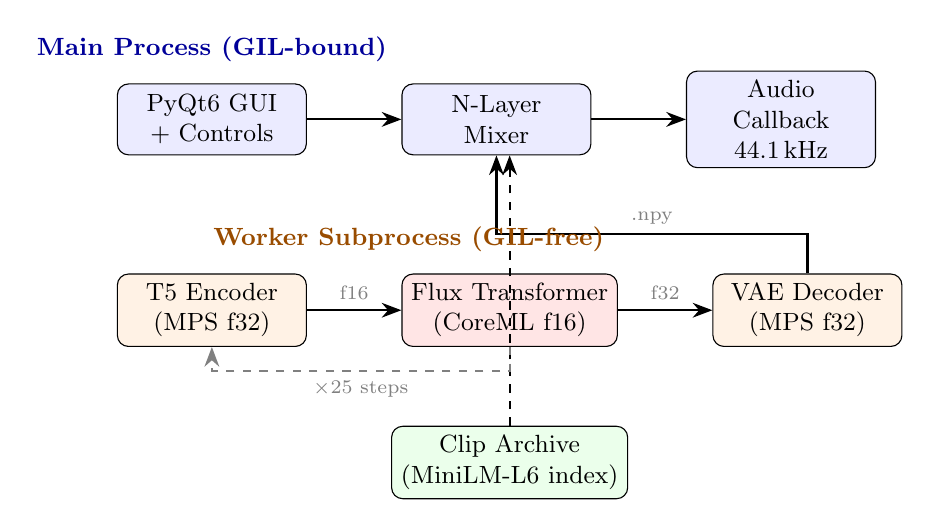
\begin{tikzpicture}[
    node distance=0.6cm and 1.2cm,
    block/.style={rectangle, draw, rounded corners, minimum height=0.9cm, minimum width=2.4cm, align=center, font=\small},
    arrow/.style={-{Stealth[length=2.5mm]}, thick},
    label/.style={font=\scriptsize, text=gray}
]
% Main process
\node[block, fill=blue!8] (gui) {PyQt6 GUI\\+ Controls};
\node[block, fill=blue!8, right=of gui] (mixer) {N-Layer\\Mixer};
\node[block, fill=blue!8, right=of mixer] (audio) {Audio\\Callback\\44.1\,kHz};

% Worker subprocess
\node[block, fill=orange!10, below=1.5cm of gui] (t5) {T5 Encoder\\(MPS f32)};
\node[block, fill=red!10, right=of t5] (flux) {Flux Transformer\\(CoreML f16)};
\node[block, fill=orange!10, right=of flux] (vae) {VAE Decoder\\(MPS f32)};

% Archive
\node[block, fill=green!8, below=1.0cm of flux] (archive) {Clip Archive\\(MiniLM-L6 index)};

% Arrows
\draw[arrow] (gui) -- (mixer);
\draw[arrow] (mixer) -- (audio);
\draw[arrow] (t5) -- node[above, label] {f16} (flux);
\draw[arrow] (flux) -- node[above, label] {f32} (vae);
\draw[arrow] (vae.north) -- ++(0, 0.5) -| node[near start, above, label] {.npy} (mixer.south);
\draw[arrow, dashed] (archive) -- (mixer.south -| archive);

% Labels
\node[above=0.15cm of gui, font=\small\bfseries, text=blue!60!black] {Main Process (GIL-bound)};
\node[above=0.15cm of t5, font=\small\bfseries, text=orange!60!black, xshift=2.5cm] {Worker Subprocess (GIL-free)};

% Scheduler loop
\draw[arrow, gray, dashed] (flux.south) -- ++(0,-0.3) -| node[below, label, pos=0.25] {$\times 25$ steps} (t5.south);
\end{tikzpicture}
\caption{System architecture of TangoFlux Endless. The inference pipeline runs in a separate subprocess to avoid GIL contention with the audio callback. The FluxTransformer2DModel is executed via CoreML (ANE/GPU, float16), while T5 encoding and VAE decoding remain in PyTorch (MPS, float32). Generated clips are exchanged as \texttt{.npy} files via a temporary directory.}
\label{fig:architecture}
\end{figure}

\subsection{Hybrid Inference Pipeline}

The TangoFlux inference pipeline consists of three stages:

\begin{enumerate}
\item \textbf{Text encoding}: Flan-T5-Large encodes the text prompt into \texttt{encoder\_hidden\_states} and \texttt{pooled\_projection} tensors (PyTorch, MPS, float32).
\item \textbf{Flow-matching denoising}: The FluxTransformer2DModel iteratively denoises latent representations over 25 Euler steps using the FlowMatchEulerDiscreteScheduler (CoreML, ANE/GPU, internally float16).
\item \textbf{Waveform decoding}: AutoencoderOobleck decodes the final latents to a 44.1\,kHz waveform (PyTorch, MPS, float32).
\end{enumerate}

The hybrid design exploits CoreML's ANE/GPU scheduling for the computationally dominant transformer while keeping the T5 encoder and VAE decoder in PyTorch MPS, which avoids the overhead of converting models with variable-length text inputs.

\subsection{Subprocess Isolation}

Python's Global Interpreter Lock (GIL) causes CPU-bound PyTorch inference and I/O-bound audio callbacks to contend for execution time.
In a threaded model, this produces audible pop/click artifacts at callback deadlines.
We eliminate GIL contention by running the generator in a separate process via \texttt{subprocess.Popen}, communicating through \texttt{.npy} files in a shared temporary directory.

\subsection{N-Layer Staggered Crossfade}

Multiple audio clips ($N=3$ by default) play simultaneously with staggered phase offsets.
Each clip uses $\sin^2/\cos^2$ fade envelopes:
\begin{equation}
\text{env}(t) = \begin{cases}
\sin^2\!\left(\frac{\pi t}{2 T_f}\right) & t < T_f \text{ (fade-in)} \\
1 & T_f \leq t \leq T - T_f \text{ (sustain)} \\
\cos^2\!\left(\frac{\pi (t - T + T_f)}{2 T_f}\right) & t > T - T_f \text{ (fade-out)}
\end{cases}
\label{eq:envelope}
\end{equation}
where $T$ is the clip duration and $T_f$ is the fade duration.
The output is normalized by $1/N$ to prevent clipping:
\begin{equation}
y(t) = \frac{1}{N} \sum_{i=1}^{N} x_i(t) \cdot \text{env}_i(t - \phi_i)
\label{eq:mixer}
\end{equation}
where $\phi_i$ is the phase offset for layer $i$.

\subsection{Archive Fallback}

When generation cannot keep pace with playback (buffer underrun), the system retrieves previously generated clips using semantic similarity.
Current prompt embeddings (all-MiniLM-L6-v2, 384-dim~\cite{reimers2019sentencebert}) are compared against an archive index via cosine similarity, and a random selection from the top-3 candidates ensures variety.

% ============================================================
\section{CoreML Conversion of Flux RoPE}
\label{sec:coreml}

The primary technical contribution is the CoreML-compatible conversion of TangoFlux's FluxTransformer2DModel.
The standard Flux implementation~\cite{esser2024sd3} contains two operations incompatible with CoreML's \texttt{coremltools.convert()} tracing:

\paragraph{Problem 1: Ellipsis \texttt{einsum}.}
The RoPE frequency computation uses:
\begin{verbatim}
  out = torch.einsum("...n,d->...nd", pos, omega)
\end{verbatim}
CoreML's tracing infrastructure (\texttt{coremltools} 8.x) cannot handle ellipsis notation in \texttt{einsum} operations.

\paragraph{Solution:}
Replace with equivalent basic tensor operations:
\begin{verbatim}
  out = pos.unsqueeze(-1) * omega.unsqueeze(0).unsqueeze(0)
\end{verbatim}

\paragraph{Problem 2: Rank-6 tensors.}
The original RoPE applies rotation via a $2\times2$ matrix representation:
\begin{verbatim}
  stacked = torch.stack([cos, -sin, sin, cos], dim=-1)
  out = rearrange(out, "b n d (i j) -> b n d i j", i=2, j=2)
  return emb.unsqueeze(1)  # rank 6!
\end{verbatim}
CoreML limits tensors to rank~5.

\paragraph{Solution:}
Separate the rotation into $(\cos, \sin)$ components and apply directly:
\begin{align}
\texttt{rope}(\mathbf{p}, d, \theta) &\rightarrow (\cos(\mathbf{p} \cdot \boldsymbol{\omega}),\; \sin(\mathbf{p} \cdot \boldsymbol{\omega})) \label{eq:rope} \\
\texttt{apply\_rope}(\mathbf{x}, \mathbf{c}, \mathbf{s}) &: \mathbf{x}_\text{out} = [\mathbf{c} \cdot x_r - \mathbf{s} \cdot x_i,\; \mathbf{s} \cdot x_r + \mathbf{c} \cdot x_i] \label{eq:apply_rope}
\end{align}
where $x_r, x_i$ denote the real and imaginary components of the paired RoPE dimensions.
This representation maintains a maximum tensor rank of~5.

\paragraph{Verification.}
We verify numerical equivalence by comparing traced outputs before and after refactoring on identical inputs.
The maximum absolute difference is $0.00$, confirming that the refactoring is lossless.

% ============================================================
\section{Experiments}
\label{sec:experiments}

All experiments are conducted on an Apple Mac Studio with M2~Ultra (24-core CPU, 76-core GPU, 32-core Neural Engine, 192\,GB unified memory) running macOS~15.3, PyTorch~2.4.0, and \texttt{coremltools}~8.1.

\subsection{Latency: CoreML vs.\ MPS}

Table~\ref{tab:latency} reports generation latency for 18-second audio clips at 25 denoising steps, measured over 10 runs after 2 warmup iterations.

\begin{table}[h]
\centering
\caption{Generation latency for 18\,s audio at 25 steps (10 runs, 2 warmup discarded).}
\label{tab:latency}
\begin{tabular}{lcccccc}
\toprule
Backend & Mean (s) & Std (s) & Min (s) & Max (s) & P95 (s) & RTF \\
\midrule
MPS (f32) & 8.049 & 0.273 & 7.652 & 8.350 & 8.328 & 0.447$\times$ \\
\textbf{CoreML (f16)} & \textbf{5.059} & 0.397 & 4.749 & 5.765 & 5.699 & \textbf{0.281$\times$} \\
\midrule
\multicolumn{4}{l}{Speedup (MPS $\div$ CoreML)} & \multicolumn{3}{r}{\textbf{1.59$\times$}} \\
\bottomrule
\end{tabular}
\end{table}

CoreML achieves a mean RTF of $0.281\times$, meaning generation completes in 28.1\% of the audio's real-time duration.
The $1.59\times$ speedup over MPS comes from ANE/GPU hybrid execution of the transformer's matrix operations, which dominate the 25-step denoising loop.

\subsection{Step Count Sweep}

Table~\ref{tab:steps} shows generation time and spectral characteristics as a function of denoising steps, using the CoreML backend.

\begin{table}[h]
\centering
\caption{Step count sweep (CoreML backend, 5 runs each). Spectral metrics computed on generated audio for the prompt ``A gentle rain falling on leaves with distant thunder.''}
\label{tab:steps}
\begin{tabular}{rcccccc}
\toprule
Steps & Time (s) & RTF & RMS & Centroid (Hz) & Flatness & Silence \\
\midrule
10 & 2.827 & 0.157$\times$ & 0.033 & 1467 & 0.054 & 0.000 \\
15 & 3.552 & 0.197$\times$ & 0.057 & 897 & 0.027 & 0.000 \\
20 & 4.252 & 0.236$\times$ & 0.060 & 623 & 0.015 & 0.000 \\
\textbf{25} & \textbf{5.003} & \textbf{0.278$\times$} & 0.057 & 1412 & 0.038 & 0.000 \\
30 & 5.900 & 0.328$\times$ & 0.048 & 2562 & 0.026 & 0.000 \\
50 & 8.898 & 0.494$\times$ & 0.058 & 775 & 0.189 & 0.167 \\
\bottomrule
\end{tabular}
\end{table}

Generation time scales linearly with step count ($\approx 0.18$\,s/step), consistent with the flow-matching Euler scheduler performing one transformer forward pass per step.
The default 25 steps offers the best trade-off: sufficient quality (low flatness, zero silence ratio) while maintaining RTF~$<0.3\times$.
At 50 steps, a silence ratio of 16.7\% emerges along with elevated spectral flatness (0.189), suggesting over-denoising.

\subsection{Prompt Variance}

Table~\ref{tab:prompts} evaluates generation consistency across five semantically distinct prompts, with 3 runs each using the CoreML backend at 25 steps.

\begin{table}[h]
\centering
\caption{Prompt variance analysis (CoreML, 25 steps, 3 runs per prompt).}
\label{tab:prompts}
\begin{tabular}{p{4.8cm}ccccc}
\toprule
Prompt & Time (s) & RTF & RMS & Centroid (Hz) & Silence \\
\midrule
Rain + thunder & 4.960 & 0.276$\times$ & 0.050 & 1183 & 0.000 \\
Ocean waves + seagulls & 5.205 & 0.289$\times$ & 0.084 & 670 & 0.034 \\
Busy caf\'{e} & 5.004 & 0.278$\times$ & 0.079 & 627 & 0.000 \\
Wind + birdsong & 4.999 & 0.278$\times$ & 0.044 & 347 & 0.061 \\
Campfire & 5.118 & 0.284$\times$ & 0.022 & 869 & 0.198 \\
\midrule
\textbf{Mean $\pm$ Std} & $5.06 \pm 0.10$ & $0.281\times$ & --- & --- & --- \\
\bottomrule
\end{tabular}
\end{table}

\textbf{Latency is prompt-independent}: the standard deviation across prompts is only 0.10\,s (2.0\% of mean), confirming that the fixed-shape CoreML model produces deterministic computation time regardless of semantic content.
In contrast, \textbf{spectral characteristics vary significantly by prompt}: RMS ranges from 0.022 (campfire) to 0.084 (ocean waves), and spectral centroid spans 347--1183\,Hz, reflecting the model's ability to produce acoustically diverse outputs.

\subsection{Spectral Analysis}

The spectral analysis reveals content-appropriate acoustic signatures:
\begin{itemize}
\item \textbf{Ocean waves} (highest RMS 0.084, centroid 670\,Hz): broadband energy distribution consistent with surf sounds.
\item \textbf{Wind + birdsong} (lowest centroid 347\,Hz): low-frequency dominance characteristic of wind with narrow tonal components.
\item \textbf{Campfire} (highest silence ratio 0.198, lowest RMS 0.022): intermittent crackling pattern with quiet intervals, acoustically appropriate for campfire sounds.
\item \textbf{Rain} (highest centroid 1183\,Hz): high-frequency energy consistent with rain noise spectrum.
\end{itemize}

% ============================================================
\section{Negative Results}
\label{sec:negative}

We document two negative results that inform future TTA deployment efforts.

\subsection{Float16 on MPS Produces Audible Artifacts}

Attempting float16 inference on Apple's MPS backend produces audible electrical noise artifacts.
The root cause is TangoFlux's \texttt{inference\_flow()} method, which creates hardcoded float32 intermediate tensors:
\begin{verbatim}
  torch.tensor(float("nan"))   # float32
  torch.randn(...)              # float32
  torch.zeros(...)              # float32
\end{verbatim}
These mix with float16 model weights during the 25-step denoising loop, causing dtype promotion mismatches.
The iterative nature of flow matching amplifies small precision errors at each step.

CoreML's internal float16 (via \texttt{compute\_precision=ct.precision.FLOAT16}) does not exhibit this problem because the CoreML runtime manages precision conversions internally, without Python-level tensor dtype conflicts.

\subsection{Disabling Classifier-Free Guidance}

Setting \texttt{guidance\_scale=0} (no CFG) reduces per-step computation but severely degrades text adherence.
Generated audio becomes generic ambient noise unrelated to the prompt.
Combined with float16 on MPS, CFG removal produces compound quality degradation.

% ============================================================
\section{Discussion}
\label{sec:discussion}

\paragraph{Comparison with GPU-side SOTA.}
FlashAudio~\cite{flashaudio2024} achieves 400$\times$ real-time on RTX~4090 with one-step generation.
Our system achieves $3.6\times$ real-time on Apple Silicon---two orders of magnitude slower in absolute terms, but operating on consumer hardware without discrete GPU.
The comparison highlights that on-device deployment on Apple Silicon is viable for real-time applications (RTF~$<1.0$) but cannot match datacenter GPU throughput.

\paragraph{Future acceleration paths.}
Several techniques could further reduce our RTF:
(1)~Latent Consistency Model distillation~\cite{luo2023lcm} to reduce the 25-step loop to 2--4 steps, potentially achieving RTF~$<0.1\times$;
(2)~mixed-bit palettization~\cite{apple2024coreml} (4-bit weights) to reduce memory bandwidth and enable more ANE parallelism;
(3)~\texttt{torch.compile} with Metal backend, currently immature but promising for future PyTorch releases.

\paragraph{Limitations.}
Our system currently generates fixed-duration 18\,s clips and achieves continuous playback through crossfade rather than true streaming generation.
The $\sim$5\,s generation latency creates a startup delay before first audio output.
The archive fallback adds variety but cannot produce truly novel content when the generator falls behind.

% ============================================================
\section{Conclusion}
\label{sec:conclusion}

We have demonstrated that real-time text-to-audio generation on Apple Silicon is achievable through a combination of CoreML conversion, subprocess isolation, and staggered crossfade playback.
Our CoreML-compatible RoPE refactoring enables deployment of Flux-architecture transformers on the Apple Neural Engine, achieving a $1.59\times$ speedup over MPS with an RTF of $0.281\times$.
The negative result on float16 MPS inference provides guidance for future TTA deployment efforts.
We release all source code, patches, and benchmark data to support reproducible research at the intersection of generative audio and edge deployment.

% ============================================================
\section*{Acknowledgments}

This work is part of \emph{Keisanki no Shizen} (Computational Nature), an installation at the National Museum of Emerging Science and Innovation (Miraikan), Tokyo.
The author thanks the Digital Nature Group at the University of Tsukuba and Pixie Dust Technologies for their support.

% ============================================================
\bibliographystyle{unsrt}
\bibliography{references}

\end{document}
